\documentclass[a4paper, 12pt]{article}
  \usepackage{cmap}
  \usepackage[unicode]{hyperref}
  \usepackage[T2A]{fontenc}
  \usepackage[utf8]{inputenc}
  \usepackage{graphicx}
    \graphicspath{{../img/}{../../img/}}
  \usepackage[usenames,dvipsnames]{xcolor}
  \usepackage[left=20mm,right=15mm,top=15mm,bottom=20mm,bindingoffset=0cm]{geometry}
  \usepackage[protrusion=true,expansion]{microtype}
  \usepackage{enumitem}
    \setlist{nolistsep} % Убираем отступы в списке
  \usepackage[compact]{titlesec}  % Контроль заголовков:
    \titlespacing{\section}{0pt}{0pt}{0pt} % - без отступов
    \titleformat*{\subsubsection}{\bfseries\itshape} % - subsubsection курсивом

  \setlength\parindent{0pt} % Убираем абзацный отступ
  \pagestyle{empty} % Убираем номера страниц

  % обёртка для списка пар "поле:значение" (например, пол:мужской),
  % используется в комплекте с командой \field
  % (текущая реализация через tabular, но может быть легко изменена)
  % TODO действительно, попробовать сделать через description как в http://tex.stackexchange.com/q/33817/24732
  \newenvironment{fieldset}%
    {\begin{tabular}{ll}}%
    {\end{tabular}}
  % пара "поле:значение" внутри \begin{fieldset}, например \field{Пол}{мужской}
  % (текущая реализация через строку в таблице и добавление двоеточия, но может быть легко изменена)
  \newcommand{\field}[2]{ #1: & #2 \\ }

  % участок с отступом слева
  \newenvironment{indented}%
    { \begingroup %
        \noindent %
        \leftskip1em}%
    { \par\endgroup }

  % запись об образовании. Четыре последовательных параметра:
  % #1 - название вуза, факультета, кафедры
  % #2 - годы обучения
  % #3 - результат (степень, награды и т.п.), может быть пустым
  % #4 - средний балл (число, например 4.5)
  \newcommand{\education}[4]{
    \par\emph{#1}

    \begin{indented}
      #2. #3\\
      Cumulative Grade Point Average: #4 out of 5.
    \end{indented}
    \vspace{1mm} % TODO переопределить в терминах parskip или типа того
  }

  % Установка полей author и title
  \newcommand{\thetitle}{Resume}
  \newcommand{\theauthor}{Ivan Novikov}
  \newcommand{\themail}{nia.afti@gmail.com}
  \author{\theauthor}
  \title{\thetitle}
  \hypersetup{
    colorlinks=true, % true: раскрашивать саму ссылку, а не рисовать
    urlcolor=Blue,
    pdfinfo={
      Title = {\thetitle},
      Author = {\theauthor (\themail)},
      Subject = {}
    }
  }

\begin{document}

  \begin{minipage}[h]{0.8\linewidth}
    \section*{\theauthor}

    \begin{fieldset}
      \field{Date of birth} {14 December 1990}
      \field{Gender}        {male}
      \field{Marital status}{single}
      \field{Address}       {16 Nevkipelogo St., apt. 177, Krasnodar, Russia}
      \field{Phone}         {+7 960 4-789-879}
      \field{E-mail}        {\href{mailto:\themail}{\nolinkurl{\themail}}}
    \end{fieldset}
  \end{minipage}
  \begin{minipage}[h]{0.19\linewidth}
    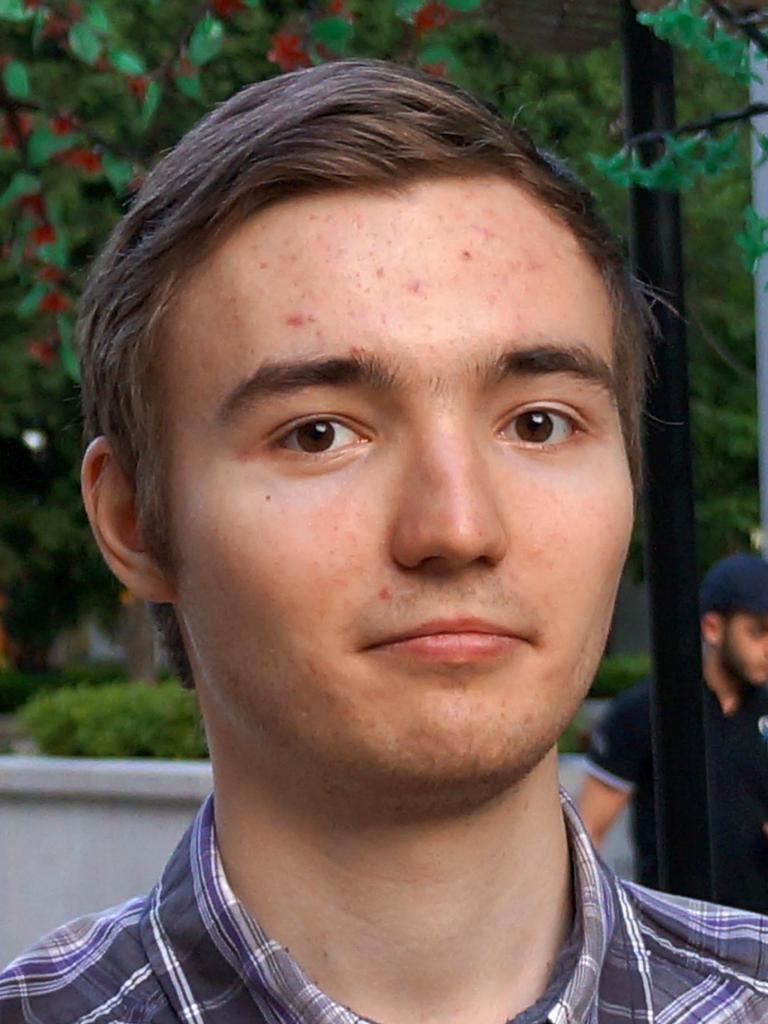
\includegraphics[width=3cm]{photo}
  \end{minipage}

  \subsection*{Education}

  \education{Kuban State University, Faculty of Physics and Technology, Physics and Informatics chair}
            {2012 — 2014}{Master of Science in Physics, diploma with honours degree.}{5.0}
  \education{Novosibirsk State University, Physics Department, Physicotechnical Research Automation chair}
            {2007 — 2011}{Bachelor of Science in Physics, diploma with honours degree.}{5.0}
  \education{``Physics and Mathematics School'' (Specialized Educational Scientific Center of NSU)}
            {2005 — 2007}{Finished with Silver Medal. Prize-winner of regional physics olympiad.}{4.9}

  English level: fluent, experienced in reading technical literature and documentation.

  \subsection*{Skills}

  Programming languages:

  \begin{itemize}[itemsep=1.5mm,topsep=2mm]
    \item[--] С, С++, Java (have been learning and using for a long time);
    \item[--] Ruby, Python (used in some educational and homebrew projects);
    \item[--] C\#, Scala (superficially acquainted, still learning).
  \end{itemize}

  Used different version control systems \emph{(Git, Subversion, Mercurial)}, relational database
  management systems \emph{(MySQL, PostgreSQL)}, web development frameworks \emph{(Ruby on Rails, Rack, Play)}.

  \subsection*{Software development experience}

  \subsubsection*{``Crash And Squeeze'' (bachelor's project + grant project)}
  \begin{description}[labelindent=1em] % TODO копипаста стиля, разобраться с этим
    \item[Topic:] ``Modeling plastic deformations of biological objects in real-time''
    \item[Company:] SoftLab-NSK (\url{http://softlab-nsk.com}): 2010 -- 2011, grant: 2013 -- present
    \item[Description:] a library to be integrated into a computer game or a virtual reality application
    \item[Source code:] \url{https://github.com/NIA/crash-and-squeeze}
    \item[Technologies and tools:] C++, DirectX 11; Google Test, Visual Studio, Git
  \end{description}

  % TODO Добавить программу по магистерскому диплому (seismoreg)?

  \subsubsection*{``Personal medical manager''}
  \begin{description}[labelindent=1em]
    \item[Position:] software engineer
    \item[Company:] NPF Mezon LLC (\url{http://mezon-kuban.ru}): 2012 -- 2014
    \item[Description:] web application to organize medical information and communicate with doctors
    \item[Website:] \url{http://diary-health.ru}
    \item[Technologies and tools:] Java, Play Framework, PostgreSQL; IntelliJ IDEA, GitHub
  \end{description}

  \subsubsection*{UGENE Assembly Browser}
  \begin{description}[labelindent=1em]
    \item[Position:] software engineer
    \item[Company:] UniPro (\url{http://unipro.ru/eng}): 2011 -- 2012
    \item[Description:] visualization of huge amounts of data in an open-source bioinformatics suite
    \item[Website:] \url{http://ugene.unipro.ru}
    \item[Technologies and tools:] C++, Qt, sqlite; Qt Creator, Subversion, JIRA, JetBrains TeamCity
  \end{description}

\end{document}
